\subsection{Problem Hardness}
\label{subsec:hard}

In this section, we show that the problem of determining whether $S^+$ accepts
sniffer trace $Tr$ is NP-complete.
%
In fact, the problem is still NP-complete
even with only one type of augmented transitions.

Recall that Type-1 transitions are added because the sniffer may miss packets.
%
Suppose there is a special sniffer that is able to capture every packet
transmitted in the communication medium.
%
In this case, there is no need to add Type-1 transitions.
%
However, Type-2 transitions are still needed since the sniffer may overhear
packets sent to the DUT.
%
Similarly, suppose another special sniffer that would not overhear any packets
sent to the DUT. That is, when this sniffer observes receiving packets, the DUT
must also have received the packet.
%
Therefore, Type-2 transitions are no longer
needed.


We refer the augmented state machine that only have Type-0 and Type-1
transitions as $S^+_1$, and the augmented state machine only have Type-0 and
Type-2 transitions as $S^+_2$.
%
Now we show that each subproblem of determining trace satisfiability is
NP-complete.

\begin{problem}
  VALIDATION-1\\
  Given that $Tr\setminus Tr_{DUT}=\emptyset$.\\
  \textbf{instance} Checker state machine $S$ and sniffer trace $Tr$.\\
  \textbf{question} Does $S^+_1$ accept $Tr$?
\end{problem}

\begin{problem}
  VALIDATION-2\\
  Given that $Tr_{DUT} \subset Tr$.\\
  \textbf{instance} Checker state machine $S$ and sniffer trace $Tr$.\\
  \textbf{question} Does $S^+_2$ accept $Tr$?
\end{problem}

To prove the following Lemma, we use a slightly extended monitor model where
boolean variables are allowed but can only be set to \texttt{true} or
\texttt{false} along state transitions. This extension makes the representation
of the state machine more succinct yet does not change the complexity of the
model, since the boolean variable assignments do not reply on the packet
payload.

\begin{lemma}
  Both VALIDATION-1 and VALIDATION-2 are NP-complete.
\end{lemma}
\begin{proof}
  First, note that the length of mutation trace $Tr'$ is polynomial to the
  length of $Tr$ because of the discrete time stamp and non-overlapping packets
  assumption.
  %
  Therefore, given a state transition sequence as witness, it can be verified in
  polynomial time whether or not it is an accepting transition sequence, hence
  both VALIDATION-1 and VALIDATION-2 are in NP.

  Next, we show how the SAT problem can be reduced to either one of the two
  problems.
  %
  Consider an instance of SAT problem of a propositional formula $F$ with $n$
  variables $x_0,x_1,\ldots, x_{n-1}$, we construct a corresponding protocol and
  its checker state machine as follows.

  The protocol involves two devices: the DUT (transmitter) and the endpoint
  (receiver).
  %
  The DUT shall send a series of packets, $pkt_0, pkt_1,\ldots, pkt_{n-1}$.
  %
  For each $pkt_i$, if the DUT receives the
  acknowledgment packet $ack_i$ from the endpoint, it sets boolean variable
  $x_i$ to be \texttt{true}.
  %
  Otherwise $x_i$ remains to be \texttt{false}.
  %
  After $n$ rounds, the DUT evaluate the formula $F$ using the assignments and
  sends a special packet, $pkt_{true}$, if $F$ is \texttt{true}.
  %
  One round of the protocol operation can be completed in polynomial time since
  any witness of $F$ can be evaluated in polynomial time.

  The protocol checker state machine $S$ is shown in Figure~\ref{fig:sat}.
  %
  Initially, all $x_i$ is set to \texttt{false}.
  %
  At state $s_0$, the DUT shall transmit $pkt_i$ within a unit time, transit to
  $s_1$ and reset the clock along the transition.
  At state $s_1$, either the DUT receives the $ack_i$ packet and
  set $x_i$ to be \texttt{true} ($s_1 \rightarrow s_0$), or the DUT continues to
  transmit the next packet $pkt_{i+1}$.
  %
  After $n$ rounds, the state machine is $s_0$ or $s_1$ depending on whether
  $ack_{n-1}$ is received by the DUT.
  %
  In either case, the DUT shall evaluate $F$ and transmit $pkt_{true}$ if $F$ is
  \texttt{true}.  

  Consider a sniffer trace $Tr_1=\{(0, pkt_0), (2, pkt_1),\\ (4,
  pkt_2),\ldots, (2(n-1), pkt_{n-1}), (2n, pkt_{true})\}$.
  %
  That is, the sniffer only captures all $pkt_i$ plus the final $pkt_{true}$, but none of
  $ack_i$.
  %
  It is easy to see that $F$ is satisfiable if $S_1^+$ accepts
  $Tr_1$.
  %
  In particular, a successful run of $S_1^+$ on $Tr_1$ would have to
  guess, for each $pkt_i$, whether the Type-1 empty transitions should be used
  to infer the missing $ack_i$ packet, such that $F$ is \textit{true} at the
  end.
  %
  Note that for $Tr_1$, no Type-2 self transitions can be used since all
  packets in $Tr_1$ are sent from the DUT.
  %
  Therefore, the SAT problem of $F$ can be reduced to the VALIDATION-1 problem
  of $S^+_1$ on sniffer trace $Tr_1$.

  \sloppy{%
    On the other hand, consider another sniffer trace $Tr_2 =\{(0, pkt_0), (1,
      ack_0), (2, pkt_1), (3, ack_1),\ldots, (2n-2, pkt_{n-1}), (2n-1, ack_{n-1}), (2n,
    pkt_{true}\}$. That is, the sniffer captures all $n$ pair of $pkt_i$ and $ack_i$
    packets and the final $pkt_{true}$ packet.  Similar to $Tr_1$, $F$ is
    satisfiable if $S^+_2$ accepts $Tr_2$. A successful transition sequence of
    $S^+_2$ on $Tr_2$ must decide for each $ack_i$ packet, whether Type-2 self
    transitions should be used, so that $F$ can be evaluated as true at the end.
    Therefore, the SAT problem of $F$ can also be reduced to the VALIDATION-2
    problem of $S^+_2$ on sniffer trace $Tr_2$.
  }

  Since SAT is known to be NP-complete, both the VALIDATION-1 and the
  VALIDATION-2 problem are also NP-complete.
\end{proof}

We now turn to the general validation problem with normal sniffers that could
either miss or overhear packets.

\begin{figure}[t]
  \centering
  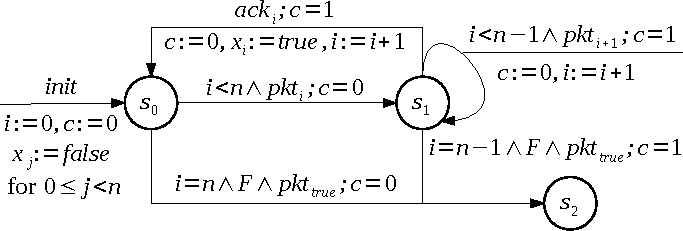
\includegraphics[width=0.48\textwidth]{./figures/sat_sm.pdf}
  \caption{\textbf{Checker State Machine for SAT Problem.}}
  \label{fig:sat}
\end{figure}



\begin{problem}
  VALIDATION\\
  \textbf{instance} Checker state machine $S$ and sniffer trace $Tr$.\\
  \textbf{question} Does $S^+$ accept $Tr$?
\end{problem}

\begin{theorem}
  VALIDATION is NP-complete.
\end{theorem}
\begin{proof}
  Based on the same reasoning that VALIDATION-1 and VALIDATION-2 are
  in NP, VALIDATION is also in NP. Furthermore, it is easy to see that both
  VALIDATION-1 and VALIDATION-2 are special instances of
  VALIDATION. Therefore, VALIDATION is NP-complete.
\end{proof}
